\documentclass[border=12pt]{standalone}
\def\pgfsysdriver{pgfsys-dvisvgm.def}
\usepackage[dvisvgm]{xcolor}
\usepackage{xeCJK}
\setCJKmainfont{HaranoAjiGothic-Regular.otf}[BoldFont=HaranoAjiGothic-Bold.otf]
\setCJKsansfont{HaranoAjiGothic-Regular.otf}[BoldFont=HaranoAjiGothic-Bold.otf]
\usepackage{amsmath,amssymb,tikz,lmodern}
\usetikzlibrary{arrows.meta,positioning,calc,fit,backgrounds}
\renewcommand{\familydefault}{\sfdefault}
\definecolor{ink}{HTML}{25322F}
\definecolor{green}{HTML}{246657}
\definecolor{tint}{HTML}{EEF4F0}
\definecolor{soft}{HTML}{C6D2CC}
\definecolor{muted}{HTML}{52615B}
\newif\ifJapanese
\newcommand{\Tx}[2]{\ifJapanese #1\else #2\fi}
\newcommand{\Eff}{\overline{\operatorname{Eff}}}
\newcommand{\heading}[3]{{\color{green}\bfseries #1\quad\Tx{#2}{#3}}\\[5pt]}
% A white rectangle makes the complete citation label clickable, including spaces.
\newcommand{\refurl}[2]{\special{dvisvgm:raw <a xlink:href="#1" target="_blank" rel="noopener noreferrer">}{\setlength{\fboxsep}{0pt}\colorbox{white}{\color{green}\underline{\strut #2}}}\special{dvisvgm:raw </a>}}
\newcommand{\refedge}[3]{\refurl{\csname source#1\endcsname\string##page=#2}{#3}}
\newcommand{\SF}[2]{\refedge{sf}{#1}{#2}}
% GitHub's file preview does not support PDF page fragments.
\newcommand{\LA}[2]{\refurl{\sourcela}{#2}}
\newcommand{\Sch}[2]{\refedge{sch}{#1}{#2}}
\newcommand{\PS}[2]{\refedge{ps}{#1}{#2}}
\tikzset{
 card/.style={draw=soft,fill=white,rounded corners=2pt,align=left,text=ink,font=\fontsize{10.5}{14}\selectfont,inner xsep=12pt,inner ysep=10pt,text width=14.4cm},
 half/.style={card,text width=6.45cm,minimum height=2.05cm},
 result/.style={card,draw=green,fill=tint,line width=.9pt},
 reason/.style={align=left,text=muted,font=\fontsize{9}{12}\selectfont,inner sep=0pt,text width=12.7cm},
 branchreason/.style={reason,text width=5.95cm},
 edge/.style={-{Stealth[length=2.4mm]},draw=green,line width=1pt},
 wire/.style={draw=green,line width=1pt},
}
% Keep the arrow in a dedicated left gutter; explanations never cover it.
\newcommand{\flow}[3]{
 \coordinate (#2-from) at ($(#1.south)+(-6.9,0)$);
 \coordinate (#2-to) at ($(#2.north)+(-6.9,0)$);
 \draw[edge] (#2-from)--(#2-to);
 \node[reason,anchor=west] (#2-reason) at ($(#2-from)!.5!(#2-to)+(.55,0)$) {#3};
}
\newcommand{\Cite}[2]{\refurl{\csname source#1\endcsname}{#2}}

\Japanesefalse
\newcommand{\sourceck}{https://github.com/openai/math/blob/adc7f1241b42e322a6451854ab7e4b4c146bf78a/preprints/Conditional-good-minimal-models-for-compact-Kahler-fourfolds-October-5-2026/paper.pdf}
\newcommand{\sourceoi}{https://github.com/openai/math/blob/adc7f1241b42e322a6451854ab7e4b4c146bf78a/preprints/Orbifold-and-logarithmic-Iitaka-subadditivity-September-26-2026/paper.pdf}
\newcommand{\sourcefm}{https://github.com/openai/math/blob/adc7f1241b42e322a6451854ab7e4b4c146bf78a/preprints/Finite-ordinary-minimal-model-programs-on-compact-Kahler-fourfolds-October-5-2026/paper.pdf}
\newcommand{\sourcean}{https://github.com/openai/math/blob/adc7f1241b42e322a6451854ab7e4b4c146bf78a/preprints/Abundance-after-nonvanishing-for-compact-Kahler-fourfolds-September-27-2026/paper.pdf}
\newcommand{\sourcedps}{https://arxiv.org/pdf/math/0006205v2}
\newcommand{\sourceou}{https://arxiv.org/pdf/2501.18088v1}
\newcommand{\sourcedo}{https://arxiv.org/pdf/2306.00671v4}
\newcommand{\sourcecce}{https://arxiv.org/pdf/1302.5016v3}
\begin{document}
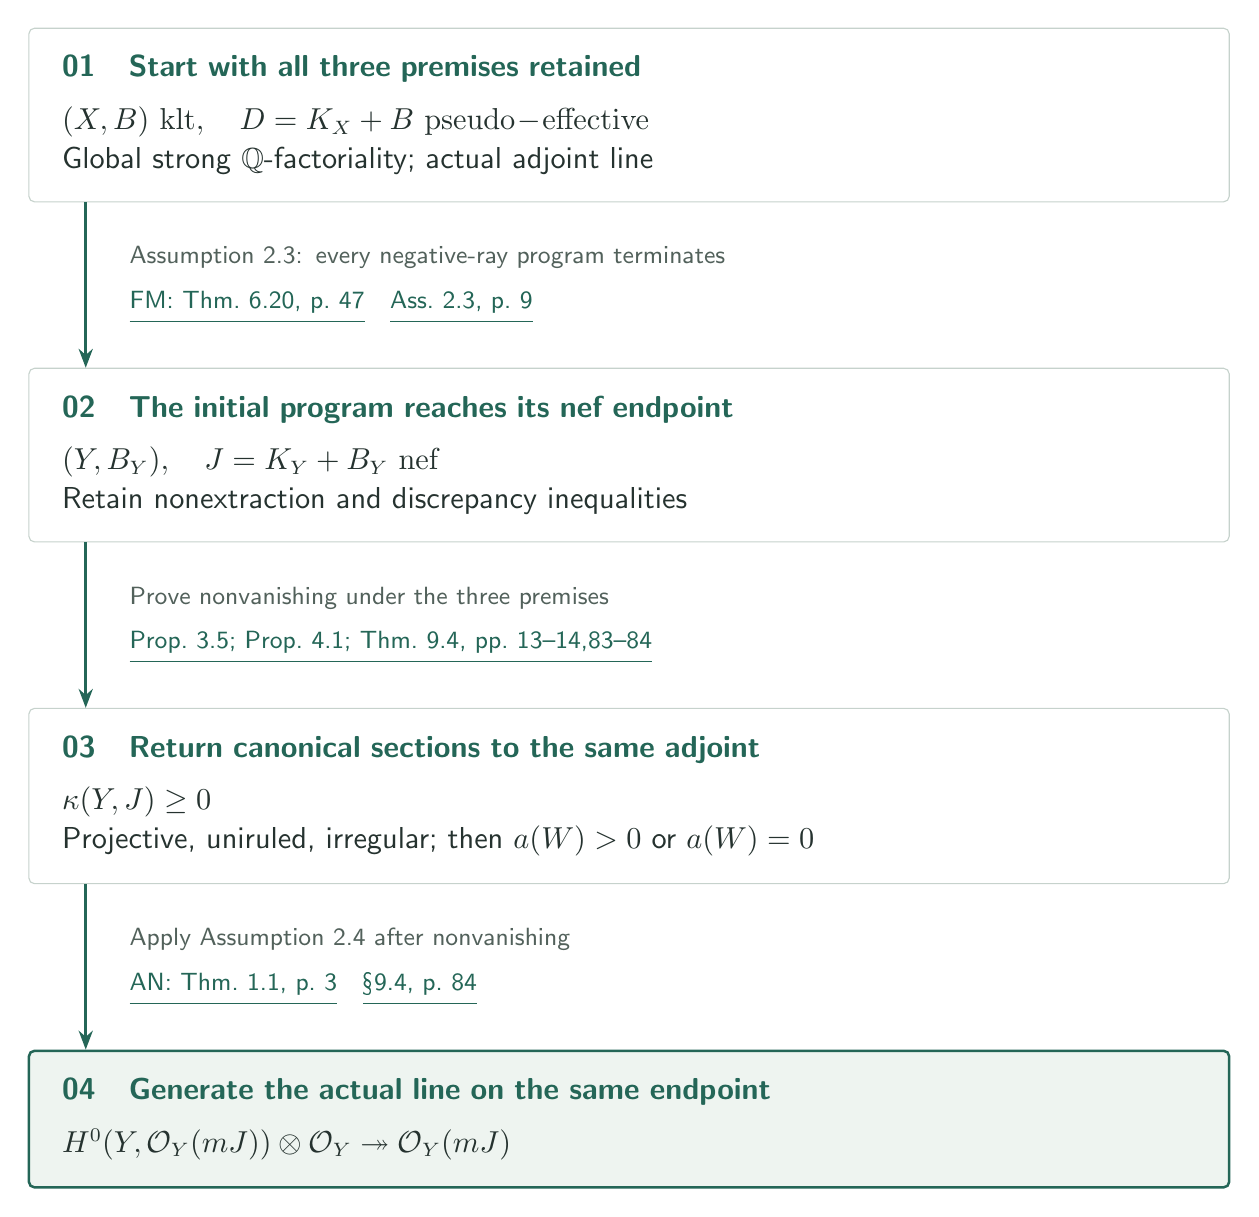
\begin{tikzpicture}
\node[card] (n0) {\heading{01}{三前提を保持した出発対}{Start with all three premises retained}\Tx{$(X,B)\ {\rm klt},\quad D=K_X+B\ {\rm pseudo\!-\!effective}$\\global strong $\mathbb Q$-factorial、実際の随伴線束}{$(X,B)\ {\rm klt},\quad D=K_X+B\ {\rm pseudo\!-\!effective}$\\Global strong $\mathbb Q$-factoriality; actual adjoint line}};
\node[card,below=2.1cm of n0] (n1) {\heading{02}{最初のプログラムのnef終点}{The initial program reaches its nef endpoint}\Tx{$(Y,B_Y),\quad J=K_Y+B_Y\ {\rm nef}$\\非抽出・discrepancy比較を保持}{$(Y,B_Y),\quad J=K_Y+B_Y\ {\rm nef}$\\Retain nonextraction and discrepancy inequalities}};
\flow{n0}{n1}{\Tx{Assumption 2.3：任意の負rayのプログラムが停止}{Assumption 2.3: every negative-ray program terminates}\\[4pt]\Cite{fm}{FM: Thm.\ 6.20, p.\ 47}\quad \Cite{ck}{Ass.\ 2.3, p.\ 9}}
\node[card,below=2.1cm of n1] (n2) {\heading{03}{canonical帰着から同じ随伴へ切断を戻す}{Return canonical sections to the same adjoint}\Tx{$\kappa(Y,J)\geq0$\\projective・uniruled・irregular、残りは $a(W)>0$ と $a(W)=0$}{$\kappa(Y,J)\geq0$\\Projective, uniruled, irregular; then $a(W)>0$ or $a(W)=0$}};
\flow{n1}{n2}{\Tx{三前提の下で非消滅を証明する}{Prove nonvanishing under the three premises}\\[4pt]\Cite{ck}{Prop.\ 3.5; Prop.\ 4.1; Thm.\ 9.4, pp.\ 13--14,83--84}}
\node[result,below=2.1cm of n2] (n3) {\heading{04}{同じnef終点の実際の線束を生成}{Generate the actual line on the same endpoint}\Tx{$H^0(Y,\mathcal O_Y(mJ))\otimes\mathcal O_Y\twoheadrightarrow\mathcal O_Y(mJ)$}{$H^0(Y,\mathcal O_Y(mJ))\otimes\mathcal O_Y\twoheadrightarrow\mathcal O_Y(mJ)$}};
\flow{n2}{n3}{\Tx{Assumption 2.4を非消滅の後で適用}{Apply Assumption 2.4 after nonvanishing}\\[4pt]\Cite{an}{AN: Thm.\ 1.1, p.\ 3}\quad \Cite{ck}{\S9.4, p.\ 84}}
\end{tikzpicture}
\end{document}
